
\documentclass[11pt]{article}
\usepackage[margin=1in]{geometry}
\usepackage{amsmath,amssymb}
\usepackage{booktabs}
\usepackage{graphicx}
\usepackage[backend=biber,style=numeric]{biblatex}
\addbibresource{references.bib}

\setlength{\parindent}{0pt}
\setlength{\parskip}{0.5\baselineskip}

\title{To What Extent Does Inlet Geometry Influence Pressure Loss Under Controlled Flow-Rate Conditions?}
\author{Rafael Kozal}
\date{\today}

\begin{document}
\maketitle

\begin{abstract}
This research plan proposes a computational fluid dynamics (CFD) study of how inlet-lip geometry affects pressure loss at a prescribed fan-face mass flow rate. Candidate axisymmetric inlet profiles will be generated from parameterised revolved sections, with the fan-face diameter, hub geometry, and operating conditions held constant. The primary performance measure will be the difference between freestream total pressure and the mass-flow-weighted mean total pressure at the fan face; total-pressure recovery and a dynamic-pressure-normalised loss will also be reported. The plan includes checks for mesh and domain sensitivity, iterative convergence, and validation against suitable benchmark or experimental data. No performance ranking is assumed before the simulations are completed.
\end{abstract}

\section{Introduction}


\subsection{Background and Rationale}
Inlet performance can be assessed using total-pressure recovery at the engine face, alongside measures of flow non-uniformity. CFD studies of engine inlets report mass-averaged fan-face total pressure relative to freestream total pressure as a recovery metric, while experimental studies also report recovery and distortion at the fan face \cite{slater2025,ybarra1981}. This plan focuses on a controlled comparison of inlet shapes rather than on a complete engine or aircraft performance assessment.

\subsection{Research Aim and Question}
The aim is to compare candidate inlet-lip profiles while holding the fan-face mass flow rate and other specified conditions constant. The research question is:
\begin{quote}
How does changing the inlet shape affect pressure loss at a measured flow rate?
\end{quote}
The initial comparison will focus on lip profile. Lip radius and inlet length may be examined in separate parameter studies so that each comparison changes one geometric factor at a time. The final set of geometries and the target mass flow rate remain to be specified.

\subsection{Hypothesis}
\emph{[State a directional prediction only after selecting the tested geometries and reviewing relevant literature. The analysis will test this prediction rather than assume that any candidate shape performs best.]}

\section{Theoretical Background}
The primary outcome will be total-pressure loss from a freestream reference station to the fan-face measurement plane. Let $p_{t,0}$ denote the freestream total pressure and let $\overline{p}_{t,2}^{\,m}$ denote the mass-flow-weighted mean total pressure at the fan face. Then
\begin{equation}
    \Delta p_t = p_{t,0} - \overline{p}_{t,2}^{\,m},
    \qquad
    \Pi_{t,\mathrm{rec}} = \frac{\overline{p}_{t,2}^{\,m}}{p_{t,0}},
    \label{eq:pressure-recovery}
\end{equation}
where $\Delta p_t$ is the total-pressure loss and $\Pi_{t,\mathrm{rec}}$ is the total-pressure recovery. The mass-flow-weighted mean on a plane $A$ is defined as
\begin{equation}
    \overline{p}_{t}^{\,m} =
    \frac{\displaystyle\int_A p_t\,\rho u_n\,\mathrm{d}A}
         {\displaystyle\int_A \rho u_n\,\mathrm{d}A},
    \label{eq:mass-weighted-pressure}
\end{equation}
where $p_t$ is local total pressure, $\rho$ is density, and $u_n$ is velocity normal to the measurement plane in the direction of flow. Reporting the loss relative to freestream dynamic pressure will support comparison across operating conditions:
\begin{equation}
    q_0 = \frac{1}{2}\rho_0 U_0^2,
    \qquad
    \Lambda_t = \frac{\Delta p_t}{q_0},
    \label{eq:normalised-loss}
\end{equation}
where $\rho_0$ and $U_0$ are freestream density and speed, respectively. Static-pressure difference is a distinct quantity and, if reported, will be identified separately rather than used interchangeably with $\Delta p_t$.

Fan-face pressure contours will be used to inspect flow non-uniformity. The maximum-minus-minimum pressure range may be reported as a supplementary descriptive statistic, but it will not be presented as a standard engine-distortion descriptor unless a recognised definition and sampling method are adopted \cite{slater2025,ybarra1981}.

\begin{center}
\begin{tabular}{lll}
\hline
\textbf{Symbol} & \textbf{Meaning} & \textbf{Unit} \\
\hline
$p_{t,0}$ & Freestream total pressure & Pa \\
$\bar{p}_{t,2}^m$ & Mass-flow-weighted mean total pressure at the fan face & Pa \\
$\Delta p_t$ & Total-pressure loss & Pa \\
$\Pi_{t,\text{rec}}$ & Total-pressure recovery & Dimensionless \\
$\rho$ & Fluid density & $\text{kg/m}^3$ \\
$u_n$ & Velocity normal to the measurement plane & m/s \\
$A$ & Measurement-plane area & $\text{m}^2$ \\
$q_0$ & Freestream dynamic pressure & Pa \\
$U_0$ & Freestream speed & m/s \\
$\Lambda_t$ & Dynamic-pressure-normalised total-pressure loss & Dimensionless \\
\hline
\end{tabular}
\end{center}

\section{Methodology}
\subsection{Experimental Design}
The study will use steady CFD simulations to compare a small set of inlet geometries at the same prescribed fan-face mass flow rate and freestream conditions. One reference geometry will be compared with three to five variants where practical. Each comparison series will vary one parameter, such as lip profile or lip radius; inlet length will be treated as a separate factor or study. The exact flow rate, fluid properties, reference dimensions, and number of geometries will be recorded before running the comparison.

\subsection{Geometry and Computational Domain}
For an axisymmetric inlet, a two-dimensional meridional profile will be parameterised and revolved about its centreline in CAD. Candidate lip profiles may include rounded and sharp forms; any ``oval'' variant will be defined precisely as either an elliptical lip cross-section or a non-circular inlet planform. The fan-face diameter, hub diameter, and all non-varied dimensions will be kept fixed. The solid inlet will be subtracted from a surrounding air volume to define the fluid domain.

The current engine assembly model is shown in Figure~\ref{fig:part-studio-1}.
\begin{figure}[htbp]
    \centering
    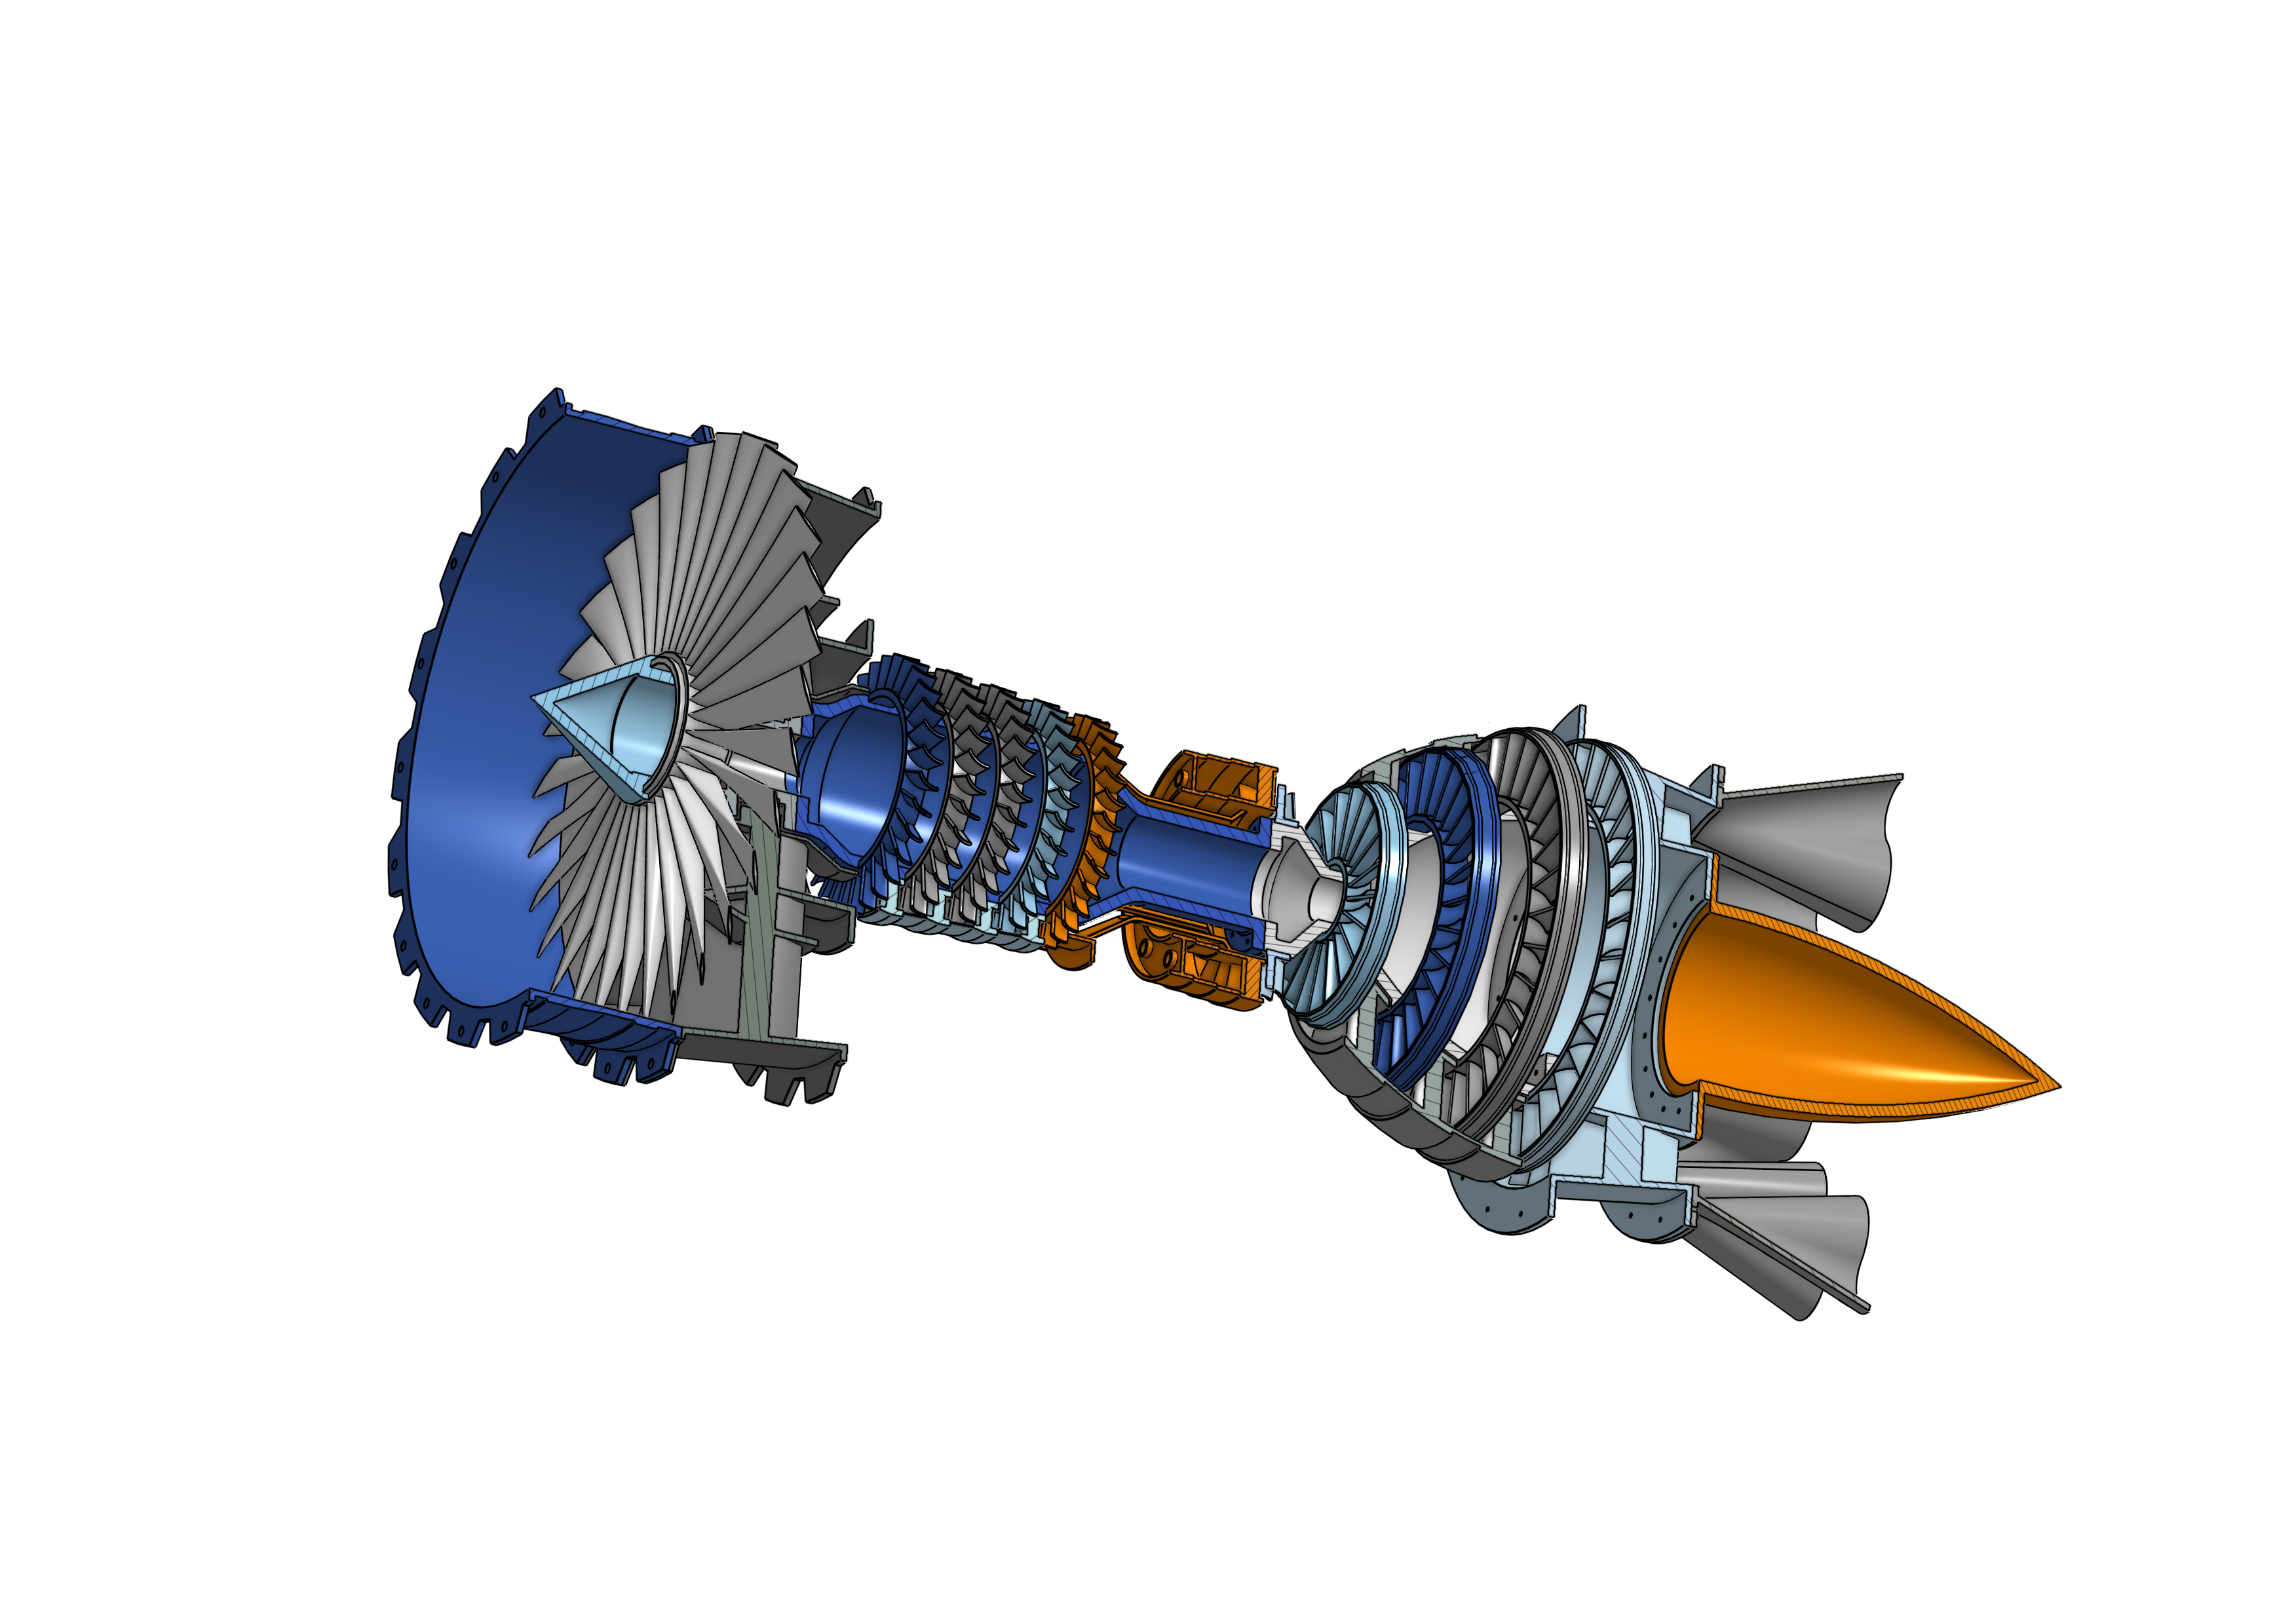
\includegraphics[width=\linewidth]{Part Studio 1.png}
    \caption{CAD rendering of the engine assembly in Part Studio 1.}
    \label{fig:part-studio-1}
\end{figure}

The upstream and lateral domain extents will be selected to represent the approach flow without materially affecting the fan-face pressure-loss result. Rather than assuming a fixed extent is sufficient, a domain-sensitivity check will compare the primary metric for successively enlarged domains. A two-dimensional axisymmetric model will be used only if the geometry, boundary conditions, and intended flow are rotationally symmetric; a non-axisymmetric planform requires a three-dimensional model.

\subsection{Solver and Boundary Conditions}
The solver, version, and available computational resources will be recorded. Candidate platforms include SimScale, Ansys Student, and OpenFOAM; final selection depends on access and the boundary-condition and post-processing features available. A steady Reynolds-averaged Navier--Stokes model is proposed as the initial approach, with the $k$--$\omega$ SST model considered as a turbulence-model candidate. The choice of turbulence model and whether air can be treated as incompressible will be justified from the operating conditions and checked against suitable evidence, rather than assumed in advance.

The upstream boundary will prescribe the selected freestream state, with appropriate far-field or pressure conditions on the outer boundaries. The same freestream conditions and fan-face mass flow will be applied to every geometry. The downstream extraction condition will be defined consistently and, where the model permits, placed beyond the fan-face measurement plane to reduce direct boundary-condition influence on that plane. The setup will avoid incompatible or duplicate constraints on a single boundary. Solver-specific boundary names and values will be documented once the software has been selected.

\subsection{Variables}
\begin{table}[htbp]
    \centering
    
    \label{tab:variables}
    \begin{tabular}{p{0.25\linewidth}p{0.19\linewidth}p{0.46\linewidth}}
        \toprule
        Variable & Role & Planned definition or control \\
        \midrule
        Lip profile or selected dimension & Independent & One geometric factor varied per comparison series \\
        Total-pressure loss, $\Delta p_t$ & Dependent & Freestream total pressure minus mass-flow-weighted fan-face total pressure (Pa) \\
        Fan-face mass flow rate & Controlled & Same target value for every geometry; specify value and unit \\
        Other controls & Controlled & Freestream state, fan-face and hub dimensions, fluid model, solver settings, and measurement-plane location \\
        \bottomrule
    \end{tabular}
    \caption{Planned CFD variables and controls.}
\end{table}

\subsection{Mesh, Convergence, and Validation}
Mesh refinement will be assessed on a representative geometry using at least three systematically refined meshes. The fan-face mass flow and primary pressure-loss metric will be monitored; a mesh will be accepted only after a predeclared tolerance for changes in the primary metric is met. Convergence assessment will consider both solver residuals and stabilisation of monitored quantities, rather than residuals alone. The domain-sensitivity study described above will check that outer-boundary placement does not dominate the comparison. These checks follow established CFD verification and validation practice, while recognising that separated flows can be particularly sensitive to physical modelling and validation data \cite{morrison2014,slater2025}.

Where suitable data are available, the baseline simulation will be compared with a benchmark case or wind-tunnel measurements, such as fan-face pressure data obtained with a Pitot probe or rake. If no matching experimental data are available, the results will be described as numerically verified to the extent tested, not as experimentally validated.

\subsection{Data Processing and Uncertainty}
For each geometry, the final converged field will be used to calculate $\Delta p_t$, $\Pi_{t,\mathrm{rec}}$, and $\Lambda_t$ using Eqs.~\ref{eq:pressure-recovery}--\ref{eq:normalised-loss}. Results will include units, the prescribed and achieved fan-face mass flow, mesh details, and the change in the primary metric under mesh and domain refinement. The pressure-resolution or numerical uncertainty must be reported relative to the observed differences; small changes will not be interpreted as meaningful if they are comparable to that uncertainty.

\section{Results}
\emph{[After completing the simulations, report the geometry dimensions, achieved mass flow rates, mesh and domain checks, and calculated pressure-loss and recovery values. Include labelled pressure and velocity contours at consistent scales. Do not report predicted values before running the CFD.]}

\section{Discussion}
\emph{[Interpret differences between geometries in relation to the research question. Use flow-field plots to examine possible separation or boundary-layer effects, compare results with cited literature, and discuss modelling assumptions, mesh sensitivity, domain sensitivity, and validation limits.]}

\section{Conclusion}
\emph{[Once results are available, answer the research question using the primary pressure-loss metric. State the size and uncertainty of the observed differences, the main limitation, and a specific next step.]}

\printbibliography[heading=bibintoc,title={References}]

\end{document}
